\documentclass[11pt]{article}
\usepackage[utf8]{inputenc}
\usepackage[T1]{fontenc}
\usepackage[final]{pdfpages} 
\usepackage[french]{babel}
\usepackage{amsmath}
\usepackage[bookmarks={true},bookmarksopen={true}]{hyperref}
\usepackage{graphicx}
\usepackage[a4paper]{geometry}
\usepackage{listings}
	\lstset{frame=tb,
		language=Java,
 		aboveskip=3mm,
  		belowskip=3mm,
  		showstringspaces=false,
  		columns=flexible,
  		basicstyle={\small\ttfamily},
  		numbers=none,
 		numberstyle=\tiny\color{gray},
  		keywordstyle=\color{blue},
  		commentstyle=\color{dkgreen},
  		stringstyle=\color{mauve},
  		breaklines=true,
  		breakatwhitespace=true
  		tabsize=3
	}
\pagestyle{plain}
\setlength{\parindent}{5mm}

\usepackage{color}

\definecolor{dkgreen}{rgb}{0,0.6,0}
\definecolor{gray}{rgb}{0.5,0.5,0.5}
\definecolor{mauve}{rgb}{0.58,0,0.82}



\title{\textbf{Projet LSINF1121 -  Algorithmique et structures de données\\ - \\ Rapport final Mission 4} \\ {\large Groupe 3.2}}
\author{Boris \bsc{Dehem} \\(5586-12-00)\and Sundeep \bsc{Dhillon} \\(6401-11-00)\and Alexandre \bsc{Hauet} \\ (5336-08-00) \and Jonathan \bsc{Powell}\\(6133-12-00)\and Mathieu \bsc{Rosar} \\ (4718-12-00)\and Tanguy \bsc{Vaessen} \\ (0810-14-00)}
\date{date}
\date{\vspace*{25mm}

\includegraphics[scale=0.75]{logo.jpg}\\
		\vspace*{30mm}
		\begin{center}
		Année académique 2014-2015 \\	
		\end{center}}

\begin{document}
\thispagestyle{empty}

\maketitle
\thispagestyle{empty}
%\tableofcontents

\newpage
\setcounter{tocdepth}{3}
\setcounter{page}{1}
\section{Introduction}

Dans le cadre du cours "Algorithmique et structures de données", il nous a été demandé de concevoir et d'implémenter une application permettant d'accéder aux informations
associées à une revue scientifique en fonction de plusieurs type de recherche et ce en implémentant une base de donnée basé à partir de \verb+Tree+.

\section{Implémentation}

La quasi-totalité du code de la mission précédente a été repris. À celui-ci quelques modifications ont été effectuées afin de tenir compte des remarques de la correction croisée. Par exemple, une exception est lancée en cas d'une ligne mal encodé. De plus nos messages d'erreurs sont maintenant affichés sur la sortie d'erreur au lieu de la sortie standard. La fonction main a été sortie de la classe \verb+Controller+ afin d'avoir un programme encore plus modulaire.

De plus deux nouvelles classes \verb+BinaryTreeSearch+ et \verb+Search+ permettent de stocker et d'aller recherche les journaux pour les différents types de champ.
\newpage
\section{Diagramme UML de classe}

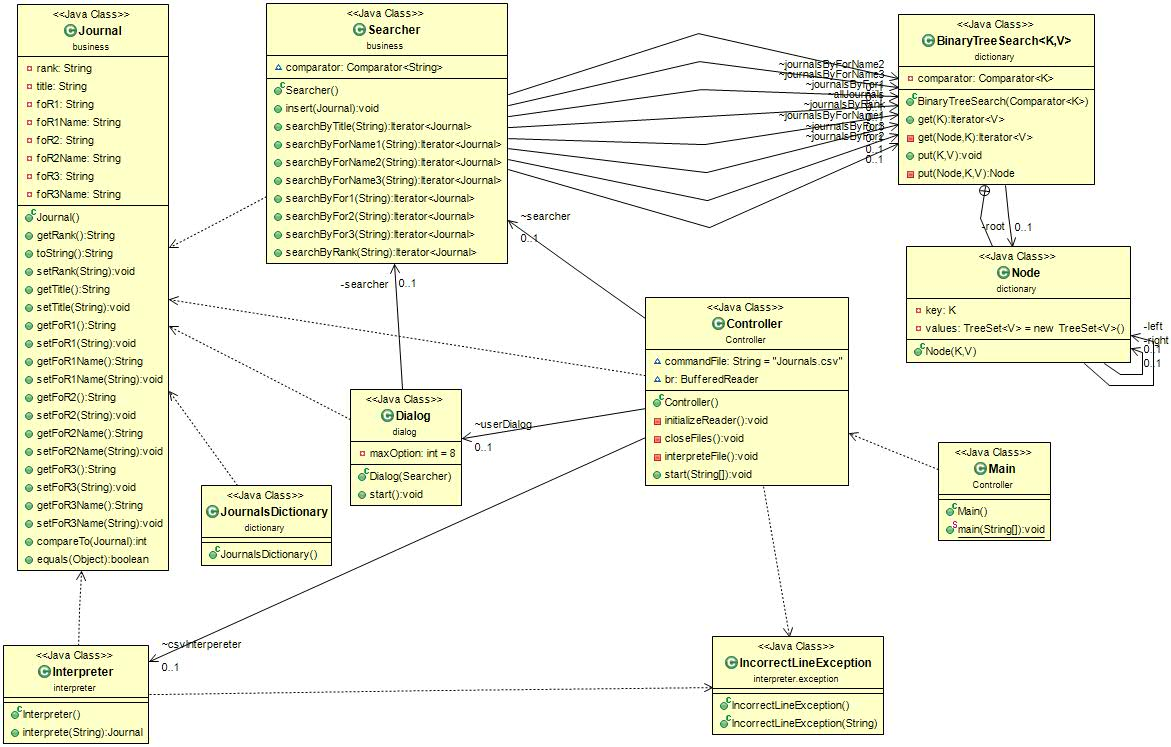
\includegraphics[width=24cm, angle=90]{dia.jpg}

\section{Questions liées au problème posé}
\subsection*{Question 9}

\subsection*{Question 10}
Étant donné que la mission précédente était fort similaire à celle-ci, il a été plus simple de se lancer dans le projet. 
La totalité des classes de l'ancienne mission ont été reprises. Certaine comme \verb+Dialogue+ a été modifié afin de correspondre aux nouvelles exigences de la mission, car désormais plusieurs types de recherches sont possibles. 

Une nouvelle classe \verb+BinaryTreeSearch+ a été ajouté afin d'obtenir par catégorie de rechercher un arbre \verb+TreeSet+ où les champs sont triés par ordre alphabétique, celle-ci remplace l'ancienne classe \verb+JournalDictionnary+

Une autre classe ajoutée est la classe \verb+Search+ qui permet de définir les huit types de recherche, un sur chaque champ du journal.

Notre mission précédente était déjà fort générique, mais à présent elle l'est encore plus. Chaque classe à sa propre tâche à effectuer. Si le besoin devient nécessaire de changer le programme en utilisant un autre type de stockage par exemple, ou une nouvelle interface pour l'utilisateur, il sera très facile pour un programmeur externe d'implémenter le code source.

Pour ce faire il peut modifier les classes qui l'intéressent et cela fonctionnera toujours sans toucher à aucune autres classes du code.

\subsection*{Question 11}

L'erreur la plus courante est le nombre incorrect de virgule dans une ligne du fichier texte. Dans le cas d'un manque de virgule la ligne est tout simplement ignorée et le programme continue de parser les autres lignes.

Il faut aussi tout particulièrement faire attention aux virgules dans la ligne de texte qui ne sont pas utilisées comme séparateur de champ, mais qui font partie du nom contenu dans ce champ.
Dans ce cas nous supposons que ces virgules se trouvent en réalité dans le titre et nous fusionnons les deux champs après le rang en un seul champ qui sera le titre.

Une autre erreur serait une ligne vide, mais nous nous retrouverons alors dans le cas de virgules manquantes

Si les champs d'une ligne sont en désordre, alors il nous est impossible de corriger cette erreur.
\end{document}

\section{Analyse de la complexité calculatoire}
\subsection{Complexité temporelle}


\section{Répartition du travail}
\begin{itemize}

\item Rédaction du rapport : Sundeep, Jonathan, Mathieu et Boris
\item Conception du programme : Tanguy, Jonathan et Alexandre.

\end{itemize}
\section{Difficultés rencontrées}

Grâce aux questions de la séance intermédiaire, nous avons décortiqué le problème ce qui nous a permis de préparer correctement le partie implémentation. Nous n'avons donc
pas rencontré de réel problème lors de la partie développement du programme. De plus la mission précédente nous a permis de partir sur de bonnes bases.